\documentclass{beamer}

\usetheme{Luebeck}

\title{Interfacing a VGA monitor with an FPGA}
\subtitle{P\&S Course iCEBreaker FPGA for IoT Sensing Systems}
\institute{ETH Zürich}
\author{Stefan Gloor}
\date{December 22, 2021}

\begin{document}

\begin{frame}
	\titlepage
\end{frame}

\begin{frame}{Goal of the project}
	\begin{itemize}
		\item Implementation of the VGA protocol
		\item Ability to display arbitrary images in color
		\item Interactive animation for demo (e.g. game)
	\end{itemize}
\end{frame}

\begin{frame}{Necessary hardware}
	\begin{minipage}{0.49\textwidth}
	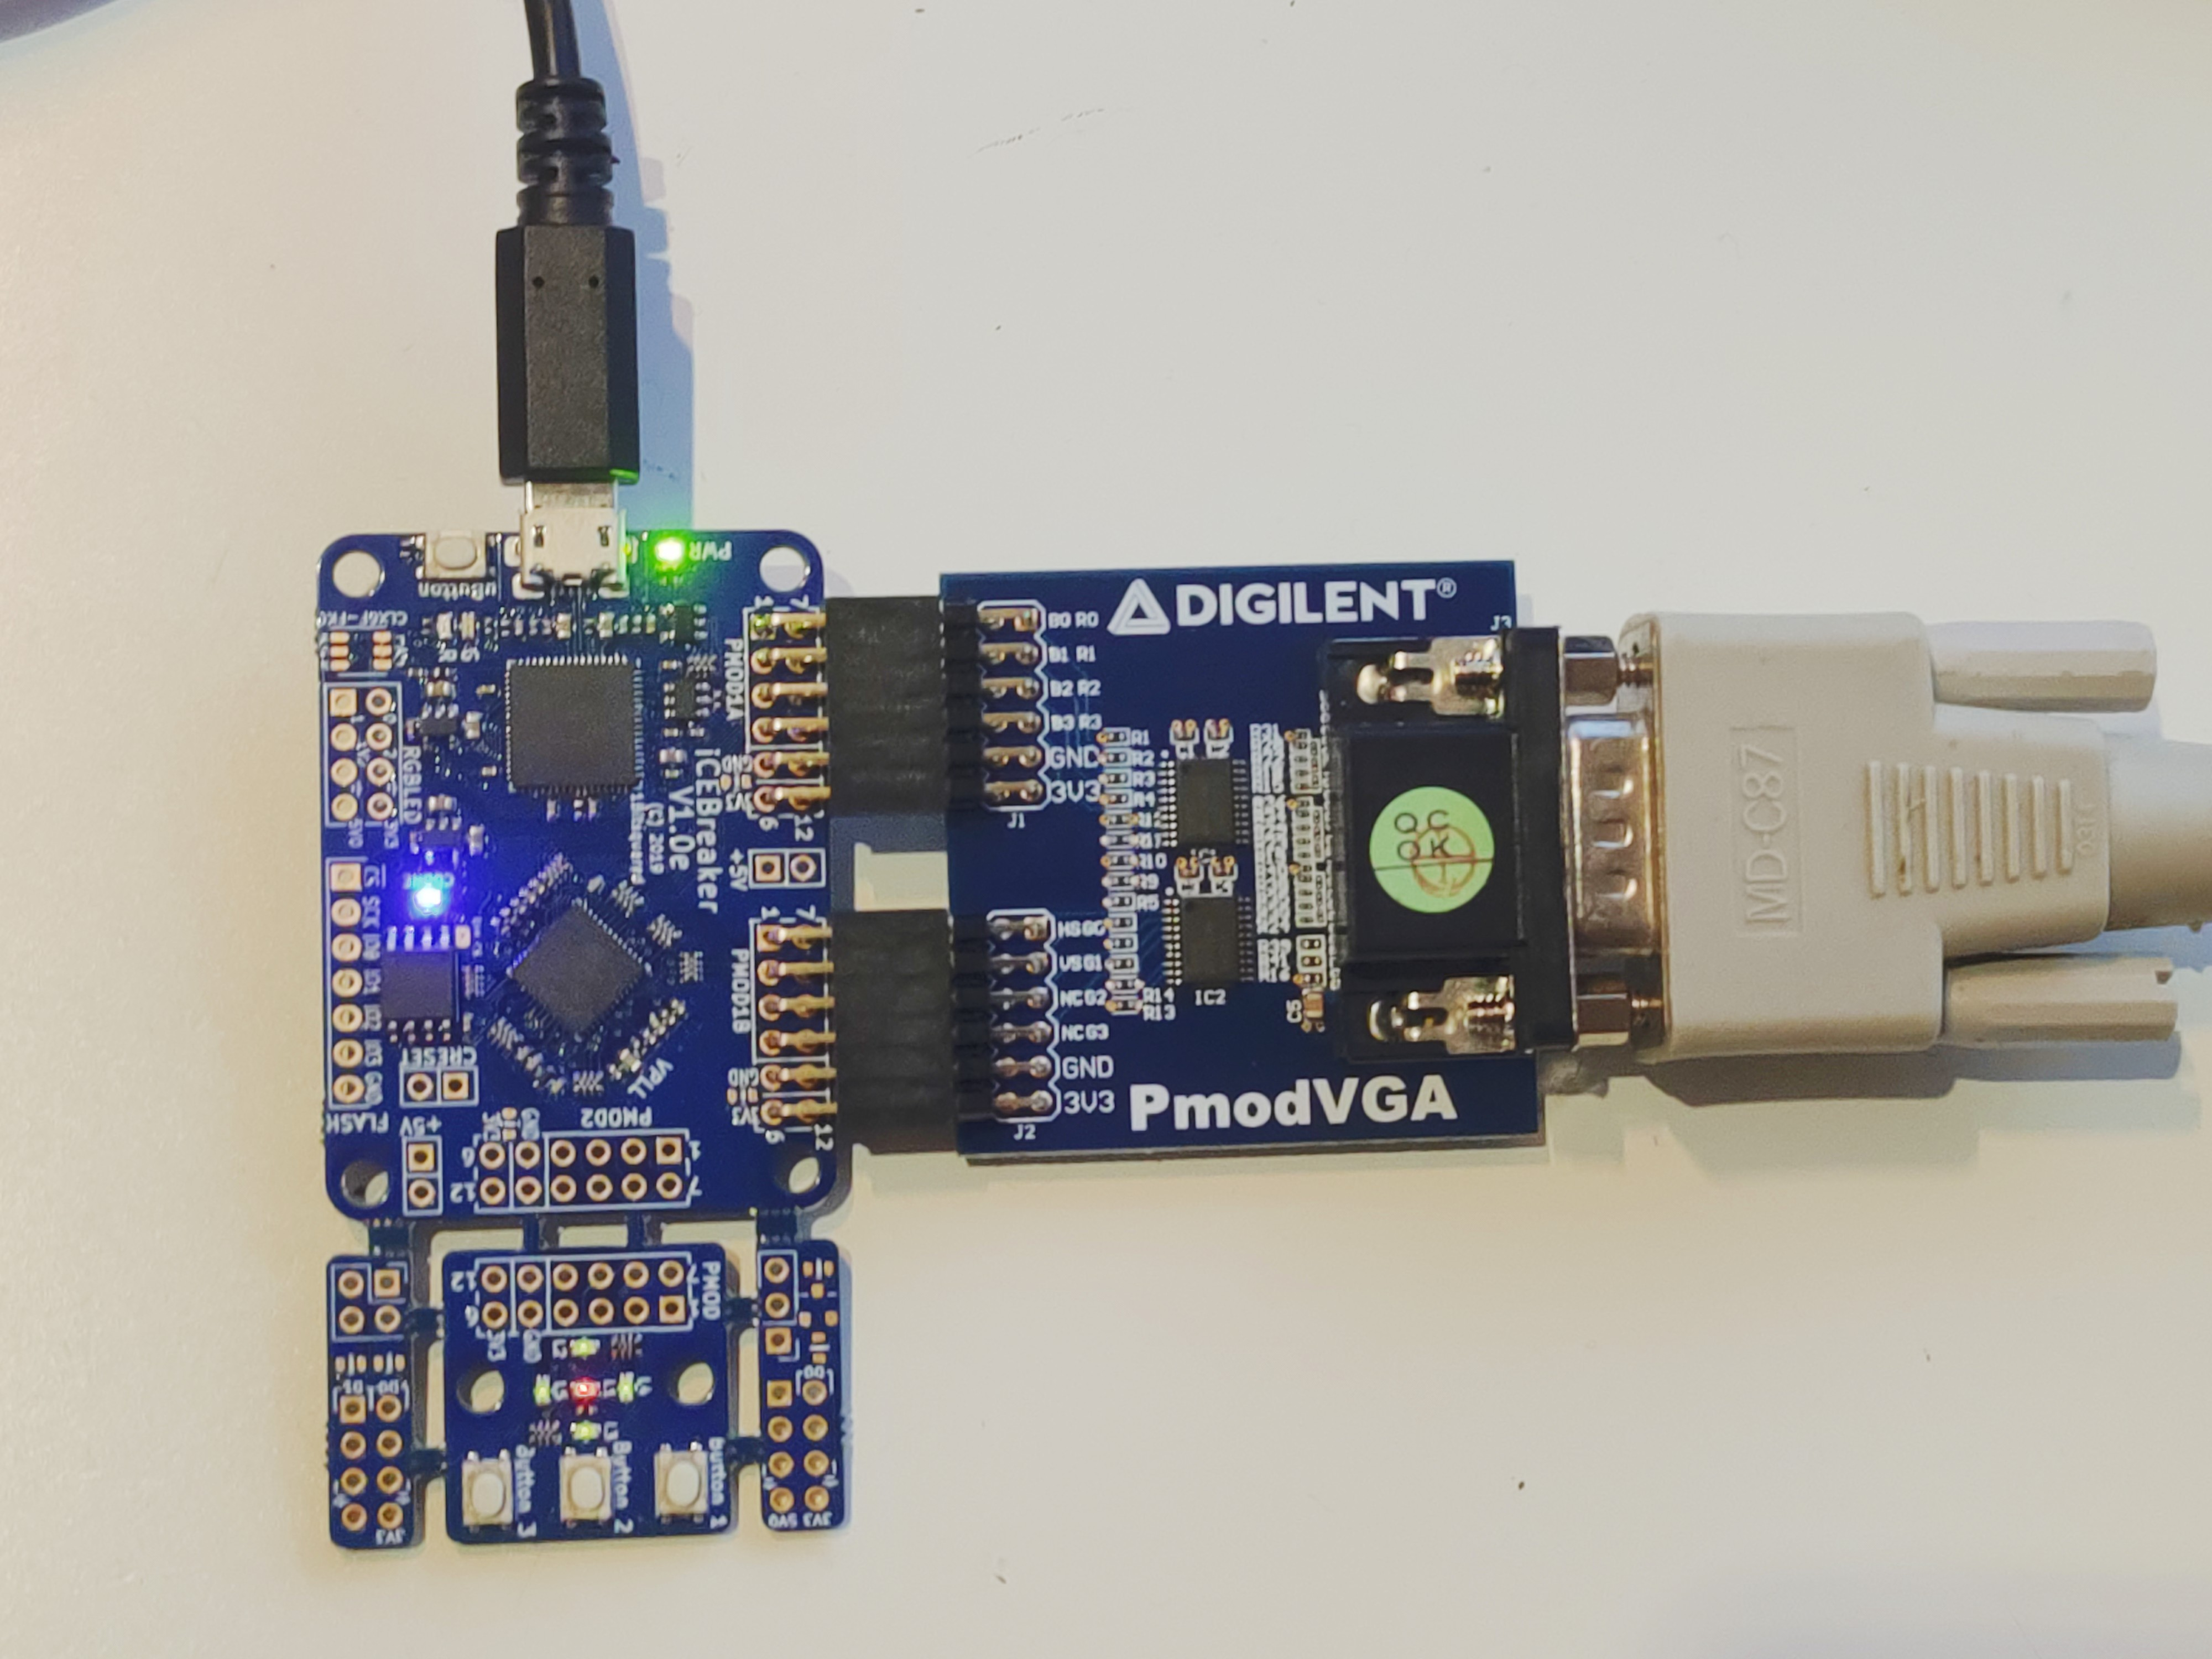
\includegraphics[width=\textwidth]{../hardware.jpg}
	\end{minipage}
	\begin{minipage}{0.49\textwidth}
		\begin{itemize}
			\item VGA Pmod
		\end{itemize}
	\end{minipage}
\end{frame}

\end{document}
